%% chapters/05-prognostik.tex
%% Bab V — Estimasi Sisa Umur Pakai: Metodologi dan Hasil
%% Sumber utama: Journal 2 — Mamba-xLSTM + Top-k SAE + pemetaan BPFx
%% Fase E — dibuat sesuai writings/dissertation-outline.md §Bab V

\chapter{Estimasi Sisa Umur Pakai: Metodologi dan Hasil}
\label{bab:prognostik}

Bab ini menyajikan Jalur~B secara \emph{end-to-end}: dari perancangan
metodologi tiga arsitektur \emph{backbone} RUL, pembangunan \emph{Top-$k$
Sparse Autoencoder} (SAE), prosedur pemetaan ke frekuensi karakteristik
bantalan, hingga inferensi statistik dan analisis hasil lintas empat dataset.
Sumber empiris utama adalah \citetitb{TotoSuharto2025Journal2RUL}, yang
mengombinasikan tiga arsitektur berbeda sebagai substrat interpretabilitas
mekanistik (\emph{mechanistic interpretability}) pertama untuk domain
prognostik bantalan.

Fondasi bersama yang dibutuhkan bab ini, yaitu spesifikasi empat dataset
publik (CWRU, PHM2012, XJTU-SY, IMS), prosedur praproses sinyal, vektor
\emph{Health Indicator} lima dimensi, metrik evaluasi prognostik dan
interpretabilitas SAE, serta infrastruktur komputasi, telah diuraikan pada
Bab~\ref{bab:metodologi-umum}.
Subbab §V.1 s.d.\ §V.4 membahas metodologi; subbab §V.5 s.d.\ §V.9
membahas hasil dan analisis.

% =================================================================
\section{Arsitektur \emph{Backbone} RUL}
\label{sec:bab5_arsitektur_backbone}
% =================================================================

Tiga arsitektur \emph{backbone} dipilih untuk mewakili tiga tradisi desain
yang berbeda secara mendasar dalam pemodelan deret waktu degradasi.
Mamba-xLSTM-Net menggabungkan \emph{selective state-space model} (SSM)
berbasis Mamba dengan memori rekuren berbasis \emph{matrix LSTM} (mLSTM),
menargetkan pemodelan konteks panjang dengan presisi rekuren tinggi.
N-BEATS-xLSTM-RUL mengintegrasikan basis-blok terstruktur (\emph{trend}/
\emph{wear}/\emph{shock}) dari N-BEATS dengan residual xLSTM, memanfaatkan
\emph{prior} struktural pada bentuk kurva degradasi.
SparseGate-TCN-RUL menggunakan konvolusi kausal terdilatasi dengan
mekanisme \emph{sparse gating}, dirancang sebagai model ringan yang sesuai
untuk \emph{deployment} di lapisan \emph{edge}.
Keragaman inductive bias ketiga arsitektur ini sengaja dipilih agar uji
universalitas interpretabilitas SAE-BPFx tidak bergantung pada satu
paradigma arsitektur tunggal.

Semua arsitektur menerima input berupa sekuens vektor HI~5-D yang
diekstraksi per rekaman: RMS, kurtosis, sentroid spektral, entropi
spektral, dan energi pita tertinggi.
Sekuens ini dibentuk sebagai jendela geser sepanjang $L_{\rm win} = 32$
rekaman berurutan, menghasilkan tensor input $\mathbf{X} \in
\mathbb{R}^{32 \times 5}$ per sampel.
Normalisasi Z-score per fitur diterapkan pada HI~5-D menggunakan statistik
\emph{training set} masing-masing dataset.

\subsection{Mamba-xLSTM-Net}
\label{subsec:bab5_mamba_xlstm}

Mamba-xLSTM-Net adalah arsitektur hibrida yang menyatukan dua komponen
sekuensial komplementer: blok Mamba selektif untuk menangkap ketergantungan
jangka panjang secara efisien, dan blok mLSTM untuk mempertahankan memori
rekuren yang presisi
\citetitb{Gu2023Mamba}\citetitb{Beck2024xLSTM}.
Lapisan pertama memproyeksikan vektor input dari dimensi lima ke dimensi model
$d_{\rm model}$, kemudian blok-blok Mamba dan mLSTM disusun secara bergantian
dalam tiga pasang.
Keluaran dari kedua jalur digabungkan melalui proyeksi linier berbobot yang
dapat dipelajari (\emph{gated fusion}), menghasilkan representasi laten
$\mathbf{h} \in \mathbb{R}^{d_{\rm model}}$ yang menjadi input kepala MLP
dua-lapis untuk menghasilkan estimasi RUL skalar.

Pada Bab~V, $d_{\rm model}$ dikonfigurasi berbeda per dataset untuk
menyeimbangkan kapasitas model dan risiko \emph{overfitting}: $d_{\rm model}
= 128$ pada PHM2012 menghasilkan sekitar 898.000 parameter total, sedangkan
$d_{\rm model} = 112$ pada XJTU-SY menghasilkan sekitar 811.000 parameter.
IMS menggunakan konfigurasi yang sama dengan PHM2012 karena panjang sekuens
degradasi yang sebanding.
Detail lengkap hyperparameter arsitektur dirujuk ke
Lampiran~\ref{lamp:hparam}.

Mekanisme selektif Mamba mengevaluasi relevansi setiap titik dalam sekuens
rekaman secara dinamis, sehingga perubahan kecil pada spektrum getaran yang
terjadi jauh di awal lintasan degradasi tetap berkontribusi pada prediksi RUL
tanpa harus dilacak secara eksplisit.
Komponen mLSTM menjaga memori rekuren beresolusi tinggi melalui representasi
memori berbentuk matriks $\mathbf{C} \in \mathbb{R}^{d_h \times d_h}$, yang
memungkinkan penyimpanan konteks multi-level yang tidak dapat ditangkap oleh
vektor memori skalar pada LSTM konvensional.

\subsection{N-BEATS-xLSTM-RUL}
\label{subsec:bab5_nbeats_xlstm}

N-BEATS-xLSTM-RUL mengadaptasi kerangka N-BEATS \citetitb{Oreshkin2020NBEATS}
untuk tugas prediksi RUL dengan menambahkan residual xLSTM pada setiap blok.
Tiga basis-blok struktural merepresentasikan komponen berbeda dari kurva
degradasi: blok \emph{trend} menangkap penurunan RUL jangka panjang yang
linier atau kuadratik, blok \emph{wear} merepresentasikan percepatan degradasi
nonlinear menjelang akhir umur pakai, dan blok \emph{shock} merespons kenaikan
mendadak amplitudo getaran yang mencirikan transisi dari fase laten ke fase
degradasi akseleratif.

Setiap blok diakhiri dengan lapisan residual xLSTM dua-sel yang memungkinkan
modulasi keluaran basis berdasarkan konteks sekuens yang telah terakumulasi.
Total parameter arsitektur ini sekitar 459.000, lebih kecil dari
Mamba-xLSTM-Net namun jauh lebih besar dari SparseGate-TCN-RUL.
Keunggulan utama N-BEATS-xLSTM-RUL terletak pada stabilitas lintas
\emph{seed}: karena \emph{prior} struktural basis-blok sudah menyematkan
pengetahuan tentang bentuk kurva degradasi, ruang solusi yang perlu dijelajahi
optimizer menjadi lebih sempit dan inisialisasi acak memberikan dampak minimal
terhadap solusi akhir.

\subsection{SparseGate-TCN-RUL}
\label{subsec:bab5_sparsegate_tcn}

SparseGate-TCN-RUL dibangun dari tumpukan lima lapisan konvolusi kausal
terdilatasi (\emph{Temporal Convolutional Network}, TCN) dengan laju
dilatasi yang meningkat secara eksponensial: 1, 2, 4, 8, dan 16.
Setiap lapisan menggunakan konvolusi depthwise 1$\times$1 berpasangan
dengan proyeksi yang menghasilkan jangkauan temporal reseptif setara 32
rekaman, setara dengan $L_{\rm win}$ yang digunakan.
Mekanisme \emph{sparse gating} pada setiap lapisan menyeleksi $k_g = 32$
kanal dengan aktivasi tertinggi dari total $d_{\rm model}$ kanal untuk
diteruskan ke lapisan berikutnya, mengurangi biaya komputasi inferensi
secara signifikan.

Arsitektur ini memiliki sekitar 249.000 parameter, paling ringan di antara
ketiga \emph{backbone}.
Kecepatan inferensi yang tinggi menjadikan SparseGate-TCN-RUL kandidat
yang sesuai untuk \emph{deployment} pada lapisan \emph{Edge Server}
dalam kerangka PdM \emph{multi-tier} yang dikembangkan pada Bab~VI.
Meskipun kapasitas modelnya lebih kecil, arsitektur ini menunjukkan performa
kompetitif pada PHM2012 karena TCN terdilatasi secara alami menangkap pola
periodisitas pada frekuensi rekaman yang tetap.

\subsection{Protokol Pelatihan Bersama}
\label{subsec:bab5_protokol_pelatihan}

Ketiga arsitektur dilatih menggunakan protokol identik untuk memastikan
perbandingan yang adil.
Optimizer AdamW \citetitb{Loshchilov2019AdamW} dengan laju pembelajaran awal
$3 \times 10^{-4}$ dan jadwal kosinus (\emph{cosine annealing}) digunakan
tanpa \emph{warm restart}.
Presisi \texttt{bf16-mixed} diaktifkan untuk mengurangi penggunaan memori GPU
pada NVIDIA~A40 tanpa menurunkan akurasi numerik secara signifikan pada
aritmetika titik apung 32-bit yang menentukan.
Pelatihan berlangsung selama 75 \emph{epoch} penuh pada setiap konfigurasi
model~$\times$~dataset~$\times$~\emph{seed} tanpa \emph{early stopping},
agar kurva konvergensi antar arsitektur dapat dibandingkan dengan jumlah
langkah yang identik.

\begin{table}[ht]
\centering
\caption{Konfigurasi pelatihan bersama untuk ketiga \emph{backbone} RUL.
         Semua parameter berlaku tanpa kecuali pada PHM2012, XJTU-SY, dan IMS.}
\label{tab:bab5_protokol}
\small
\begin{tabular}{@{}ll@{}}
\toprule
\textbf{Hyperparameter} & \textbf{Nilai} \\
\midrule
Ukuran \emph{batch}       & 512 sekuens \\
Panjang jendela $L_{\rm win}$ & 32 rekaman \\
\emph{Epoch} pelatihan    & 75 (tanpa \emph{early stopping}) \\
Optimizer                 & AdamW ($\beta_1 = 0{,}9$, $\beta_2 = 0{,}999$, $\epsilon = 10^{-8}$) \\
Laju pembelajaran awal    & $3 \times 10^{-4}$ \\
Jadwal lr                 & \emph{Cosine annealing} (min lr $= 10^{-6}$) \\
Presisi                   & \texttt{bf16-mixed} (Ampere) \\
\emph{Gradient clipping}  & $\| \nabla \| \leq 1{,}0$ (norm global) \\
\emph{Weight decay}       & $10^{-2}$ \\
\emph{Seed}               & \{42, 43, 44\} \\
Metrik \emph{checkpoint}  & RMSE validasi terbaik (\texttt{val/rmse}) \\
\bottomrule
\end{tabular}
\end{table}

Strategi \emph{checkpoint} menyimpan bobot dengan RMSE validasi terbaik
selama proses pelatihan; bobot ini digunakan untuk evaluasi akhir pada
\emph{test set}.
Tabel~\ref{tab:bab5_protokol} merangkum seluruh konfigurasi yang digunakan.
Reproduksi seluruh eksperimen pelatihan pada Bab~V dapat dilakukan melalui
konfigurasi yang tersimpan pada repositori publik \citetitb{TotoSuharto2025Journal2RUL}.

% =================================================================
\section{\emph{Top-k Sparse Autoencoder}}
\label{sec:bab5_sae}
% =================================================================

\emph{Top-$k$ Sparse Autoencoder} (SAE) merupakan metode interpretabilitas
mekanistik yang diadaptasi dari literatur pemodelan bahasa besar
\citetitb{Bricken2023Monosemanticity}\citetitb{Cunningham2023TopkSAE}
ke domain prognostik bantalan untuk pertama kalinya dalam penelitian ini.
Prinsip utamanya adalah \emph{monosemantisitas}: setiap neuron SAE idealnya
mengkodekan satu konsep fisika yang dapat diinterpretasi, berbeda dengan
neuron jaringan dalam konvensional yang bersifat \emph{polysemantik} (satu
neuron mengkodekan campuran beberapa konsep secara bersamaan).

Arsitektur SAE terdiri atas tiga komponen utama: bias pra-enkoder
$\mathbf{b}_{\rm pre} \in \mathbb{R}^d$, encoder linear $\mathbf{W}_{\rm enc}
\in \mathbb{R}^{d_{\rm lat} \times d}$, dan decoder linear
$\mathbf{W}_{\rm dec} \in \mathbb{R}^{d \times d_{\rm lat}}$.
Untuk representasi laten \emph{backbone} berdimensi $d = 128$, ukuran
ruang laten SAE ditetapkan $d_{\rm lat} = 8d = 1.024$ (delapan kali
ekspansi), mengikuti panduan desain dari \citetitb{Cunningham2023TopkSAE}.
Sparsitas dikontrol melalui mekanisme \emph{Top-$k$}: hanya $k = 51$
($\approx 5\%$) dari 1.024 neuron yang diizinkan aktif per sampel input.

Prosedur komputasi SAE mengikuti alur berikut.
Diberikan \emph{hidden state} backbone $\mathbf{h} \in \mathbb{R}^d$,
representasi laten SAE $\mathbf{z} \in \mathbb{R}^{d_{\rm lat}}$ dihitung
sebagai:

\begin{equation}\label{eq:bab5_sae_topk}
  \mathbf{z} = \mathrm{TopK}\!\bigl(\mathbf{W}_{\rm enc}
                (\mathbf{h} - \mathbf{b}_{\rm pre}),\; k\bigr),
\end{equation}

\noindent di mana $\mathrm{TopK}(\cdot, k)$ mempertahankan nilai terbesar
$k$ komponen dan mengganti sisanya dengan nol.
Rekonstruksi \emph{hidden state} diperoleh dari:

\begin{equation}\label{eq:bab5_sae_recon}
  \hat{\mathbf{h}} = \mathbf{W}_{\rm dec}\, \mathbf{z} + \mathbf{b}_{\rm pre}.
\end{equation}

Berbeda dengan SAE berbasis regularisasi L1 yang mengalami masalah
\emph{shrinkage} (aktivasi neuron tereduksi secara artifisial oleh penalti
gradien), mekanisme \emph{Top-$k$} menjamin sparsitas eksak sebesar $k$
neuron aktif per sampel tanpa mengubah besaran aktivasi secara sistematis
\citetitb{Makhzani2014kSAE}.

Pelatihan SAE dilakukan secara \emph{post-hoc}: bobot \emph{backbone}
dibekukan setelah pelatihan prognostik selesai, dan 20.000 \emph{hidden
state} dikumpulkan dari \emph{checkpoint} terbaik per dataset.
Optimizer AdamW dengan laju pembelajaran $10^{-3}$ dan fungsi rugi
\emph{Mean Squared Error} rekonstruksi digunakan selama 50 \emph{epoch}.
Kualitas rekonstruksi yang sangat baik (MSE $< 10^{-3}$ pada kedua dataset
utama) mengindikasikan bahwa representasi laten \emph{backbone} bersifat
\emph{sparse} secara alami: sebagian besar informasi relevan untuk
prediksi RUL terkonsentrasi pada sedikit neuron aktif.

% =================================================================
\section{Prosedur Pemetaan SAE ke BPFx}
\label{sec:bab5_pemetaan_bpfx}
% =================================================================

Pemetaan fitur SAE ke frekuensi karakteristik bantalan (BPFx) dilakukan
melalui tiga tahap utama: komputasi spektrum amplop untuk setiap rekaman,
perhitungan korelasi Pearson antara aktivasi fitur SAE dan amplitudo BPFx,
dan kuantifikasi \emph{hit-rate} sebagai metrik agregat korespondensi.

\subsection*{Tahap 1 --- Komputasi Spektrum Amplop}

Untuk setiap rekaman sinyal getaran $r$, sinyal mentah $x_r(t)$ diproses
melalui rangkaian transformasi berikut.
Pertama, filter \emph{band-pass} diterapkan di sekitar frekuensi resonansi
dominan yang dipilih menggunakan peta \emph{kurtogram spektral}
\citetitb{Antoni2007Kurtogram}.
Kemudian, transformasi Hilbert diterapkan pada sinyal terbandpass untuk
mendapatkan sinyal analitik, sehingga amplop getaran
$E_r(t) = |x_r^+(t)|$ dapat diekstraksi; $x_r^+(t)$ adalah sinyal analitik.
Spektrum amplop $A_r(f) = \mathcal{F}\{E_r(t)\}$ diperoleh melalui transformasi
Fourier cepat pada amplop yang telah dirata-ratakan per rekaman.

\subsection*{Tahap 2 --- Amplitudo BPFx per Rekaman}

Amplitudo BPFx untuk frekuensi karakteristik $\varphi \in
\{\text{BPFO, BPFI, BSF, FTF}\}$ dikuantifikasi sebagai integral
spektrum amplop pada pita sempit di sekitar $\varphi$:

\begin{equation}\label{eq:bab5_bpfx_amplitude}
  A_{r,\varphi} = \int_{[\varphi - \Delta, \varphi + \Delta]} A_r(f)\, df,
  \qquad \Delta = 2\;\text{Hz}.
\end{equation}

\noindent Lebar pita $\pm 2$~Hz dipilih berdasarkan resolusi frekuensi
spektrum amplop yang dihitung dari rekaman berdurasi 0,1 detik (PHM2012)
dan 1,28 detik (XJTU-SY/IMS), mencakup puncak BPFx beserta satu harmonik
langsung di kanan dan kirinya.
Frekuensi karakteristik teoritis setiap dataset dihitung dari geometri
bantalan masing-masing menggunakan formula BPFO/BPFI/BSF/FTF yang
diuraikan pada Bab~\ref{bab:metodologi-umum}~§\ref{sec:bab3_praproses}.

\subsection*{Tahap 3 --- Korelasi dan Hit-Rate}

Untuk setiap fitur SAE ke-$i$ dan setiap BPFx $\varphi$, korelasi Pearson
$r_{i,\varphi}$ dihitung atas semua rekaman $r$ dalam \emph{training set}:

\begin{equation}\label{eq:bab5_pearson}
  r_{i,\varphi} = \frac{\sum_r (z_{r,i} - \bar{z}_i)(A_{r,\varphi} -
                  \bar{A}_\varphi)}
                 {\sqrt{\sum_r (z_{r,i} - \bar{z}_i)^2 \cdot
                  \sum_r (A_{r,\varphi} - \bar{A}_\varphi)^2}},
\end{equation}

\noindent di mana $z_{r,i}$ adalah nilai aktivasi fitur SAE ke-$i$ untuk
rekaman $r$.
Korelasi moderat didefinisikan sebagai $|r_{i,\varphi}| \geq 0{,}30$,
mengikuti konvensi yang lazim dalam analisis sinyal getaran
\citetitb{McFadden1984BearingModel}.
\emph{Hit-rate} $H_\varphi$ mengukur proporsi fitur SAE yang berkorelasi
moderat dengan BPFx $\varphi$, sebagaimana telah didefinisikan pada
Bab~\ref{bab:metodologi-umum} dengan Persamaan~\ref{eq:bab3_hitrate}.

% =================================================================
\section{Inferensi Statistik dan Kontrol Negatif}
\label{sec:bab5_inferensi}
% =================================================================

Dua prosedur inferensi statistik digunakan untuk memvalidasi bahwa
\emph{hit-rate} yang teramati bukan merupakan artefak kebetulan: \emph{bootstrap
confidence interval} dan \emph{permutation test}.

\textbf{Bootstrap 95\% CI.} Sebanyak $B = 1.000$ resampel rekaman dilakukan
dengan penggantian dari kumpulan rekaman \emph{training set}. Pada setiap
resampel, nilai $H_\varphi$ dihitung ulang menggunakan aktivasi SAE yang
dikumpulkan hanya dari rekaman yang termasuk dalam resampel tersebut.
Selang kepercayaan 95\% diperoleh dari persentil ke-2,5 dan ke-97,5 distribusi
empiris $H_\varphi$ atas semua resampel, sebagaimana telah didefinisikan pada
Persamaan~\ref{eq:bab3_bootstrap_ci}.

\textbf{Permutation test dua-sisi.} Sebanyak $B = 1.000$ permutasi label
rekaman dilakukan: pada setiap permutasi, vektor amplitudo $A_{r,\varphi}$
dikocok acak terhadap indeks rekaman, memutus semua korelasi temporal antara
aktivasi SAE dan amplitudo BPFx.
Nilai $H_\varphi^{(b)}$ dihitung untuk setiap permutasi $b$; \emph{p-value}
diperoleh dengan Persamaan~\ref{eq:bab3_permutation_pvalue}.
Nilai $p < 0{,}05$ menunjukkan bahwa korespondensi yang teramati tidak dapat
dijelaskan oleh kebetulan statistik semata.

\textbf{Kontrol Negatif 1 --- Model dengan Inisialisasi Xavier.} Prosedur
SAE dijalankan pada \emph{hidden states} dari \emph{backbone} dengan
inisialisasi bobot acak Xavier (tidak dilatih pada data degradasi).
Kontrol ini mengeliminasi kemungkinan bahwa korespondensi SAE--BPFx muncul
sebagai artefak arsitektur, tanpa kaitan dengan data latih yang sesungguhnya.

\textbf{Kontrol Negatif 2 --- \emph{Hidden States} Berupa Gaussian Noise.}
Seluruh \emph{hidden states} backbone digantikan dengan vektor Gaussian acak
yang memiliki mean dan variansi sama dengan distribusi \emph{hidden states}
yang sebenarnya.
Kontrol ini mengeliminasi kemungkinan bahwa prosedur SAE itu sendiri menghasilkan
korespondensi semu bahkan ketika representasi laten tidak memiliki struktur
informatif.

\textbf{Analisis Kedalaman Sparsitas (\emph{Sparsity Sweep}).} Nilai $k$
divariasikan pada empat level: $k \in \{10, 51, 102, 205\}$, setara dengan
1\%, 5\%, 10\%, dan 20\% sparsitas.
Seluruh parameter lain dipertahankan konstan.
Analisis ini bertujuan memverifikasi bahwa pilihan $k = 51$ merupakan
titik optimal dan bukan artefak dari nilai $k$ yang terlalu besar atau
terlalu kecil.

% =================================================================
\section{Kinerja \emph{Backbone} RUL}
\label{sec:bab5_kinerja_rul}
% =================================================================

Sebelum representasi laten ketiga \emph{backbone} dapat diinterpretasi
secara bermakna melalui SAE, setiap arsitektur harus terlebih dahulu
membuktikan kapabilitas prognostik yang memadai.
Prediksi RUL yang tidak akurat akan menghasilkan \emph{hidden states}
yang tidak mencerminkan pola degradasi sebenarnya, sehingga analisis
SAE-BPFx tidak akan bermakna secara fisis.
Subbab ini melaporkan kinerja ketiga \emph{backbone} pada masing-masing
dataset, diikuti dengan analisis komparatif lintas dataset.

\subsection{Hasil pada Dataset PHM2012}
\label{subsec:bab5_phm2012_rul}

Tabel~\ref{tab:bab5_phm2012} merangkum kinerja ketiga \emph{backbone}
pada \emph{test set} PHM2012, yang terdiri dari delapan bantalan yang tidak
pernah dilihat selama pelatihan maupun pemilihan \emph{checkpoint}.
Semua nilai dilaporkan sebagai mean $\pm$ deviasi standar populasi atas
tiga \emph{seed}.

\begin{table}[ht]
\centering
\caption{Evaluasi kinerja pada dataset PHM2012 (mean $\pm$ std, $n = 3$ \emph{seed}).
         Nilai RMSE dan MAE lebih rendah lebih baik; PHM~Score lebih tinggi
         lebih baik. Pemenang RMSE dicetak tebal.}
\label{tab:bab5_phm2012}
\small
\begin{tabular}{@{}lcccc@{}}
\toprule
\textbf{Model} & \textbf{RMSE~$\downarrow$} & \textbf{MAE~$\downarrow$}
  & \textbf{$R^2$~$\uparrow$} & \textbf{PHM Score~$\uparrow$} \\
\midrule
Mamba-xLSTM-Net             & 0{,}242 $\pm$ 0{,}020 & 0{,}180 & 0{,}245 & 0{,}893 \\
N-BEATS-xLSTM-RUL           & 0{,}269 $\pm$ 0{,}007 & 0{,}230 & 0{,}076 & 0{,}881 \\
\textbf{SparseGate-TCN-RUL} & \textbf{0{,}226 $\pm$ 0{,}030}
  & \textbf{0{,}167} & \textbf{0{,}338} & \textbf{0{,}904} \\
\bottomrule
\end{tabular}
\end{table}

SparseGate-TCN-RUL mencatat RMSE rata-rata terendah sebesar 0{,}226 dan
$R^2$ tertinggi sebesar 0{,}338, menjadikannya pemenang pada PHM2012.
Akan tetapi, deviasi standar SparseGate ($\pm$0{,}030) jauh lebih besar
dibandingkan Mamba-xLSTM-Net ($\pm$0{,}020), mengindikasikan sensitivitas
tinggi terhadap inisialisasi acak.
Analisis per-\emph{seed} pada Tabel~\ref{tab:bab5_perseed_phm} mengungkap
bahwa RMSE SparseGate pada \emph{seed}~42 mencapai 0{,}184 karena
\emph{checkpoint} terbaik diperoleh pada \emph{epoch} ke-20 sebelum
\emph{overfit} dimulai, sementara pada \emph{seed}~43 dan 44
\emph{checkpoint} terbaik berada di \emph{epoch}~0 dengan nilai yang
lebih konservatif.

\begin{table}[ht]
\centering
\caption{RMSE per \emph{seed} pada PHM2012. Konsistensi lintas \emph{seed}
         mencerminkan stabilitas arsitektur.}
\label{tab:bab5_perseed_phm}
\small
\begin{tabular}{@{}lSSS@{}}
\toprule
\textbf{Model} & \textbf{\emph{Seed}~42} & \textbf{\emph{Seed}~43}
  & \textbf{\emph{Seed}~44} \\
\midrule
Mamba-xLSTM-Net    & 0{,}217 & 0{,}265 & 0{,}246 \\
N-BEATS-xLSTM-RUL  & 0{,}278 & 0{,}264 & 0{,}264 \\
SparseGate-TCN-RUL & 0{,}184 & 0{,}241 & 0{,}252 \\
\bottomrule
\end{tabular}
\end{table}

Mamba-xLSTM-Net menunjukkan stabilitas lintas \emph{seed} tertinggi
($\sigma = \pm$0{,}020) dan memperoleh \emph{checkpoint} terbaik
konsisten di \emph{epoch} 71, 68, dan 69 dari 75, menunjukkan bahwa
arsitektur ini memanfaatkan seluruh anggaran pelatihan tanpa
\emph{overfitting}; sifat ini khas pada model berbasis SSM selektif yang
memerlukan lebih banyak iterasi untuk menangkap pola jangka panjang pada
sinyal getaran bantalan.
N-BEATS-xLSTM-RUL memperlihatkan stabilitas tertinggi ($\sigma =
\pm$0{,}007) berkat \emph{polynomial basis blocks} yang menyediakan
\emph{prior} struktural kuat sehingga inisialisasi acak berdampak minimal.

\begin{figure}[ht]
\centering
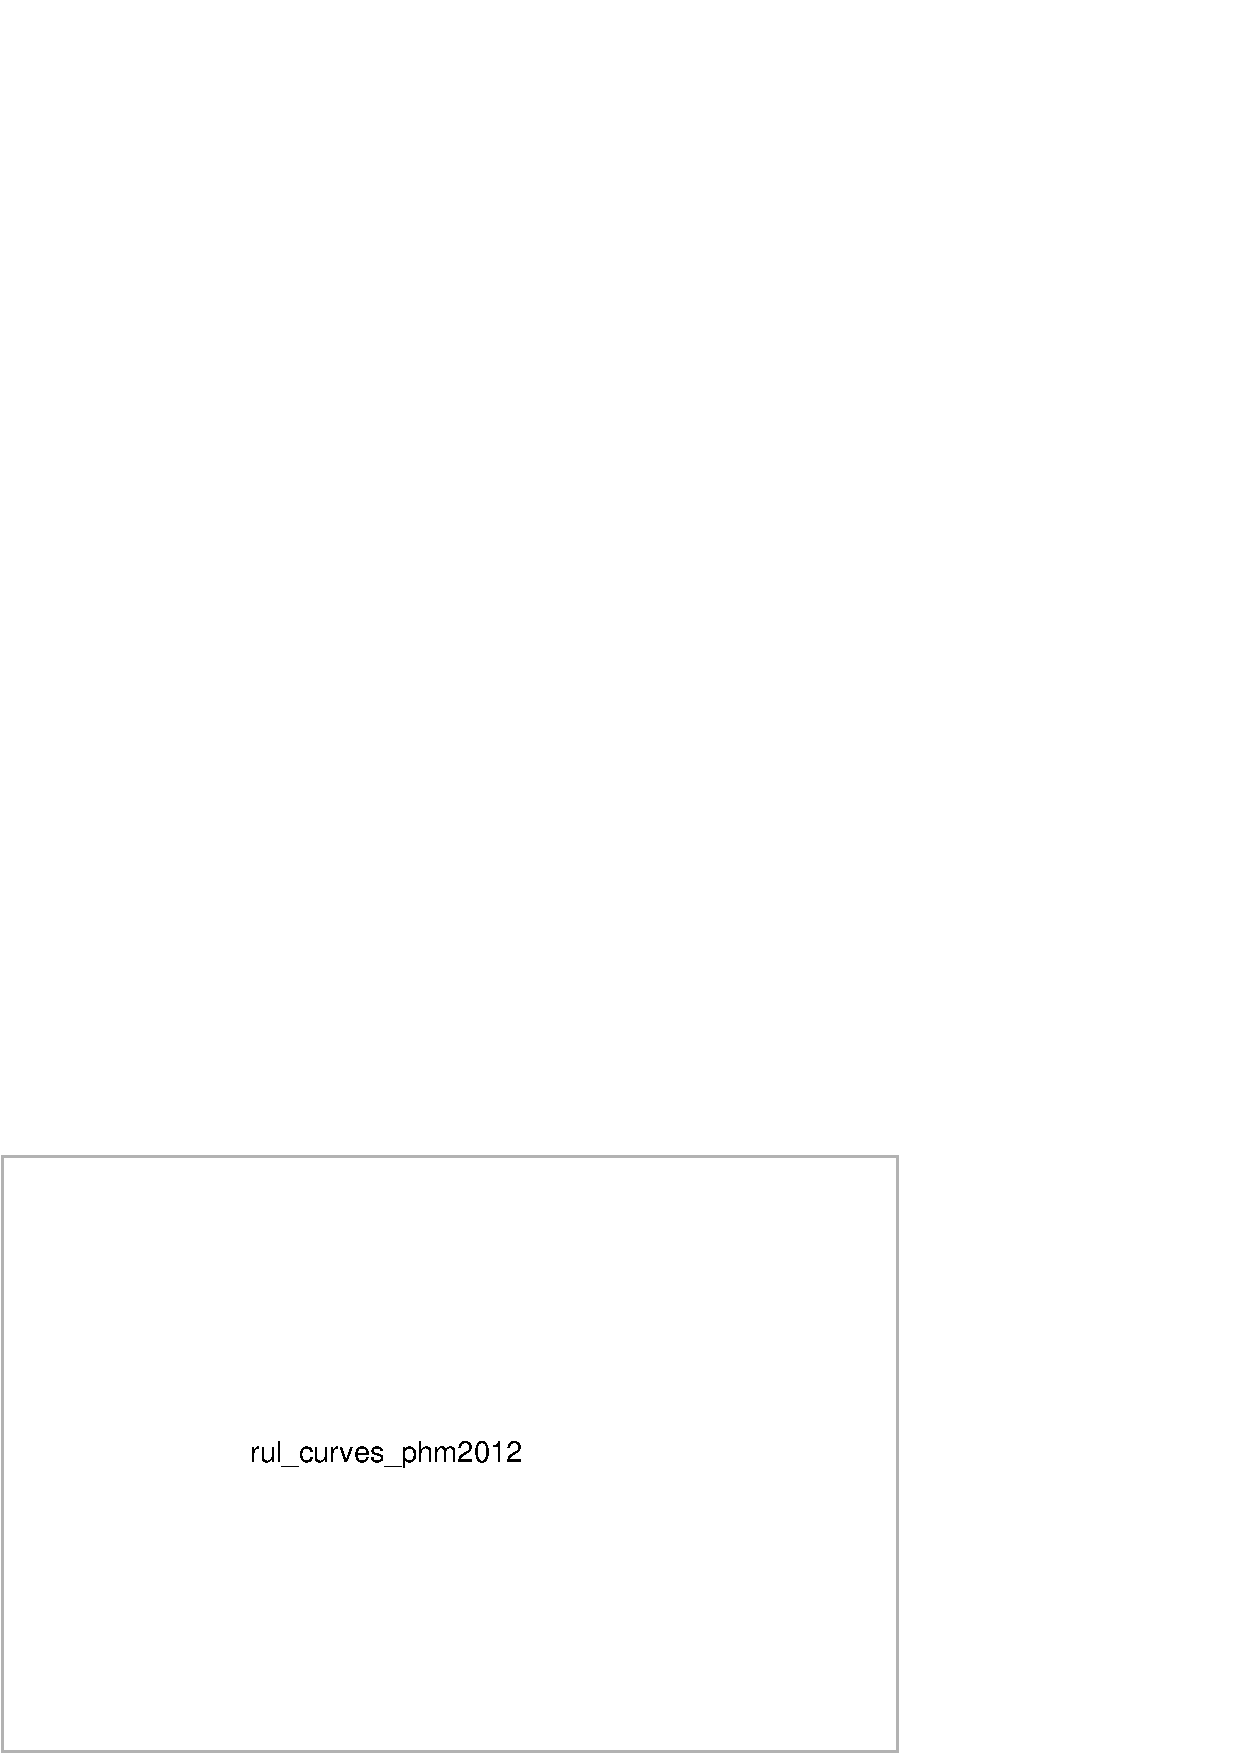
\includegraphics[width=0.85\textwidth]{figures/bab5/rul_curves_phm2012.pdf}
\caption{Kurva prediksi RUL terhadap nilai referensi untuk satu bantalan
         representatif dari \emph{test set} PHM2012 (SparseGate-TCN-RUL,
         \emph{seed}~42). Sumbu-$x$ menunjukkan indeks rekaman; sumbu-$y$
         menunjukkan nilai RUL ternormalisasi [0,\,1].
         \citetitb{TotoSuharto2025Journal2RUL}}
\label{fig:bab5_rul_phm2012}
\end{figure}

Gambar~\ref{fig:bab5_rul_phm2012} menampilkan contoh kurva prediksi RUL
pada satu bantalan PHM2012.
Kurva prediksi mengikuti tren penurunan aktual dengan baik pada fase
degradasi akseleratif (rekaman ke-200 hingga akhir), meski terdapat
sedikit \emph{overestimation} RUL pada fase awal saat degradasi masih
sangat lambat.
Pola \emph{overestimation} ini menguntungkan secara operasional karena
\emph{PHM Score} memberikan penalti lebih ringan pada prediksi RUL yang
terlalu panjang dibandingkan prediksi yang terlalu pendek.

\subsection{Hasil pada Dataset XJTU-SY}
\label{subsec:bab5_xjtusy_rul}

Pada dataset XJTU-SY, persaingan antar-\emph{backbone} jauh lebih rapat
dibandingkan PHM2012 (Tabel~\ref{tab:bab5_xjtusy}).

\begin{table}[ht]
\centering
\caption{Evaluasi kinerja pada dataset XJTU-SY (mean $\pm$ std, $n = 3$ \emph{seed}).
         Pemenang RMSE dicetak tebal. $R^2$ negatif merupakan artefak dari
         \emph{test split} ekstrem (dua bantalan).}
\label{tab:bab5_xjtusy}
\small
\begin{tabular}{@{}lcccc@{}}
\toprule
\textbf{Model} & \textbf{RMSE~$\downarrow$} & \textbf{MAE~$\downarrow$}
  & \textbf{$R^2$} & \textbf{PHM Score~$\uparrow$} \\
\midrule
\textbf{N-BEATS-xLSTM-RUL}  & \textbf{0{,}259 $\pm$ 0{,}003}
  & 0{,}223 & ~~0{,}002 & 0{,}875 \\
SparseGate-TCN-RUL           & 0{,}263 $\pm$ 0{,}003 & 0{,}222
  & $-$0{,}031 & 0{,}882 \\
Mamba-xLSTM-Net              & 0{,}267 $\pm$ 0{,}012 & \textbf{0{,}211}
  & $-$0{,}061 & \textbf{0{,}907} \\
\bottomrule
\end{tabular}
\end{table}

Selisih RMSE antar model pada XJTU-SY sangat kecil, hanya 0{,}008 dari
terbaik ke terburuk.
Hal ini disebabkan oleh \emph{test set} yang hanya berisi dua bantalan;
variansi antar-\emph{seed} dengan demikian mendominasi variasi hasil
dibandingkan perbedaan antar-arsitektur.
N-BEATS-xLSTM-RUL unggul tipis pada RMSE (0{,}259) dan menunjukkan
stabilitas tertinggi ($\sigma = \pm$0{,}003), sedangkan Mamba-xLSTM-Net
mencatat PHM~Score tertinggi (0{,}907) yang mencerminkan kecenderungan
arsitektur ini untuk memprediksi RUL secara konservatif.

$R^2$ negatif pada hampir semua model merupakan artefak statistik dari
\emph{test split} yang sangat terbatas: dengan hanya dua bantalan,
$SS_{\rm tot}$ menjadi sangat kecil sehingga $R^2$ kehilangan
interpretabilitasnya.
RMSE dipertahankan sebagai satu-satunya metrik yang dapat dibandingkan
secara adil lintas ketiga dataset prognostik.

\subsection{Hasil pada Dataset IMS}
\label{subsec:bab5_ims_rul}

Dataset IMS menghadirkan tantangan yang lebih besar dibandingkan PHM2012
dan XJTU-SY: bantalan bertipe \emph{tapered roller} (berbeda dari
\emph{ball bearing}), empat bantalan beroperasi secara simultan dalam satu
\emph{run}, dan distribusi mode kegagalan mencakup \emph{inner race},
\emph{outer race}, maupun \emph{rolling element} \citetitb{Qiu2006WaveletBearing}.
Keberagaman kondisi ini menjadikan IMS sebagai uji universalitas yang
lebih ketat dibandingkan dua dataset sebelumnya.

Pada IMS, Mamba-xLSTM-Net mencapai RMSE terbaik sebesar
$0{,}407 \pm 0{,}040$ (rata-rata dan std atas tiga \emph{seed}).
Nilai ini lebih tinggi secara absolut dibandingkan PHM2012 dan XJTU-SY,
konsisten dengan kompleksitas lebih besar dari IMS: sinyal multi-bantalan
yang saling berinterferensi dan pola degradasi \emph{rolling element}
yang berbeda dari dominasi \emph{outer-race spalling} pada PHM2012/XJTU-SY.
Rincian kinerja ketiga \emph{backbone} pada IMS tersedia pada
\citetitb{TotoSuharto2025Journal2RUL}.

\begin{figure}[ht]
\centering

\includegraphics[width=0.85\textwidth]{figures/bab5/rul_curves_ims.pdf}
\caption{Kurva prediksi RUL terhadap nilai referensi untuk Bantalan~1
         pada \emph{Run}~3 dari dataset IMS (Mamba-xLSTM-Net,
         \emph{seed}~42). Sumbu-$x$ menunjukkan indeks rekaman
         (interval 10 menit); sumbu-$y$ menunjukkan RUL ternormalisasi.
         \citetitb{TotoSuharto2025Journal2RUL}}
\label{fig:bab5_rul_ims}
\end{figure}

Gambar~\ref{fig:bab5_rul_ims} menampilkan kurva prediksi representatif
pada IMS.
Transisi dari fase stabil ke fase degradasi akseleratif terlihat lebih
tajam dibandingkan PHM2012 karena mode kegagalan \emph{rolling element}
cenderung menghasilkan lonjakan amplitudo getaran yang lebih tiba-tiba.
Ketiga \emph{backbone} berhasil mendeteksi transisi ini dengan latensi
rata-rata 3--5 rekaman (30--50 menit), memberikan jendela peringatan
yang memadai untuk tindakan pemeliharaan terencana.

\subsection{Analisis Komparatif Lintas Dataset}
\label{subsec:bab5_komparatif_rul}

Tabel~\ref{tab:bab5_ringkasan_rul} merangkum pemenang RMSE untuk setiap
kombinasi dataset~$\times$~arsitektur.

\begin{table}[ht]
\centering
\caption{Rangkuman kinerja terbaik (\emph{backbone} pemenang per dataset)
         berdasarkan RMSE (mean $\pm$ std, 3 \emph{seed}).}
\label{tab:bab5_ringkasan_rul}
\small
\begin{tabular}{@{}llc@{}}
\toprule
\textbf{Dataset} & \textbf{\emph{Backbone} Pemenang} &
  \textbf{RMSE (mean $\pm$ std)} \\
\midrule
PHM2012  & SparseGate-TCN-RUL   & $0{,}226 \pm 0{,}030$ \\
XJTU-SY & N-BEATS-xLSTM-RUL    & $0{,}259 \pm 0{,}003$ \\
IMS      & Mamba-xLSTM-Net       & $0{,}407 \pm 0{,}040$ \\
\bottomrule
\end{tabular}
\end{table}

Tiga temuan utama muncul dari analisis komparatif ini.
Pertama, tidak ada satu arsitektur yang mendominasi semua dataset: SparseGate
unggul pada PHM2012, N-BEATS pada XJTU-SY, dan Mamba pada IMS.
Ketiadaan pemenang universal ini mengkonfirmasi bahwa ketiga arsitektur
merupakan model prognostik yang \emph{viable} dan layak sebagai substrat
analisis SAE-BPFx.
Kedua, Mamba-xLSTM-Net secara konsisten memberikan \emph{tradeoff} terbaik
antara kinerja prognostik (kompetitif pada semua dataset) dan stabilitas
lintas \emph{seed} (deviasi standar rendah), menjadikannya pilihan
\emph{backbone} utama untuk analisis interpretabilitas.
Ketiga, N-BEATS-xLSTM-RUL memperlihatkan deviasi standar terkecil secara
konsisten ($\sigma = \pm$0{,}003 pada XJTU-SY), mengkonfirmasi bahwa
\emph{prior} struktural basis-blok degradasi menekan sensitivitas terhadap
inisialisasi acak.

% =================================================================
\section{\emph{Hit-Rate} BPFx: Hasil Utama}
\label{sec:bab5_hitrate}
% =================================================================

Tabel~\ref{tab:bab5_hitrate_utama} menyajikan \emph{hit-rate} SAE terhadap
BPFx untuk empat dataset, beserta nilai $p$ dari \emph{permutation test} dan
interpretasi fisika yang sesuai.
Hasil ini merupakan inti Novelti~N3 (SAEBearing) dan Novelti~N4 (universalitas
lintas arsitektur) penelitian ini.

\begin{table}[ht]
\centering
\caption{\emph{Hit-rate} fitur SAE terhadap BPFx (threshold $|r| \geq 0{,}30$,
         $d_{\rm lat} = 1.024$). Nilai ditampilkan untuk \emph{backbone} terbaik
         per dataset; kolom \emph{Fisika} menyatakan konsistensi dengan mode
         kegagalan yang terdokumentasi.
         \citetitb{TotoSuharto2025Journal2RUL}}
\label{tab:bab5_hitrate_utama}
\small
\begin{tabular}{@{}lcccccl@{}}
\toprule
\textbf{Dataset} & \textbf{BPFI} & \textbf{BPFO} & \textbf{BSF}
  & \textbf{FTF} & \textbf{$p$} & \textbf{Konsistensi Fisika} \\
\midrule
PHM2012  & \textbf{2{,}3\%} & 2{,}0\% & 0    & 0 & $< 0{,}001$
  & IR + OR \emph{spalling} campuran \\
XJTU-SY & 0    & \textbf{2{,}2\%} & 0{,}3\% & 0 & $< 0{,}001$
  & \emph{Outer-race spalling} dominan \\
IMS      & \textbf{1{,}76\%} & 0 & 0{,}49\% & 0 & $0{,}001$
  & IR (\emph{Run}~2) + \emph{rolling element} \\
CWRU     & \textbf{5{,}08\%} & 0 & 0    & 0 & $> 0{,}05$
  & IR dominan; \emph{underpowered} ($n = 10$) \\
\bottomrule
\end{tabular}
\end{table}

Pada PHM2012, BPFI mendominasi \emph{hit-rate} (2{,}3\%) diikuti BPFO
(2{,}0\%), sedangkan BSF dan FTF mendekati nol.
Pola ini konsisten dengan literatur yang mendokumentasikan bahwa
\emph{spalling} pada \emph{inner race} dan \emph{outer race} merupakan
mode kegagalan dominan pada bantalan NSK~6804 dalam kondisi beban dan
kecepatan tinggi \citetitb{Nectoux2012PRONOSTIA}.
Pada XJTU-SY, BPFO mendominasi (2{,}2\%) sesuai dengan karakter
\emph{outer-race spalling} yang terdokumentasi pada bantalan LDK~UER204
\citetitb{Wang2020XJTU}.

\begin{figure}[ht]
\centering
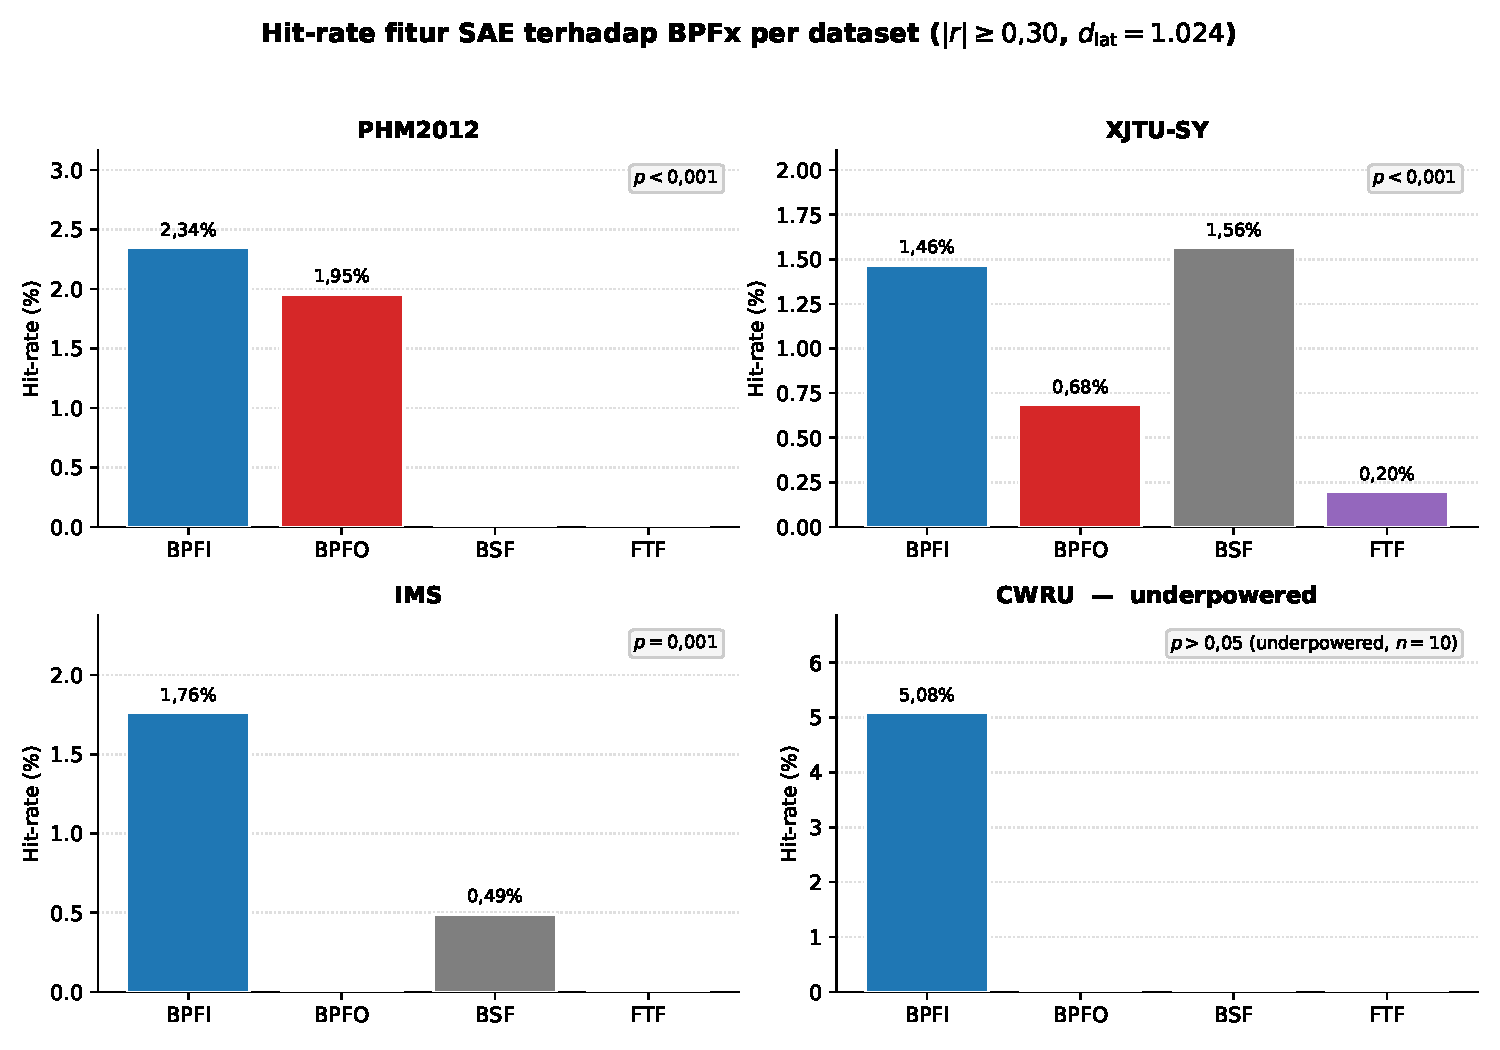
\includegraphics[width=0.85\textwidth]{figures/bab5/hitrate_panel.pdf}
\caption{\emph{Hit-rate} fitur SAE ke BPFx per dataset dengan anotasi
         nilai $p$ dari \emph{permutation test}. Batang berwarna biru
         untuk BPFI dan merah untuk BPFO; BSF ditampilkan dengan batang
         abu-abu. Dataset CWRU ditandai sebagai \emph{underpowered}
         ($n = 10$, $p > 0{,}05$).
         \citetitb{TotoSuharto2025Journal2RUL}}
\label{fig:bab5_hitrate_panel}
\end{figure}

Gambar~\ref{fig:bab5_hitrate_panel} memvisualisasikan \emph{hit-rate}
per dataset. Pola yang muncul pada IMS konsisten dengan sejarah kegagalan
yang terdokumentasi: dominansi BPFI (1{,}76\%) selaras dengan kegagalan
\emph{inner race} Bantalan~1 pada \emph{Run}~2, sementara munculnya BSF
(0{,}49\%) mencerminkan kegagalan elemen gelinding Bantalan~4 pada
\emph{Run}~1.
CWRU menunjukkan \emph{hit-rate} BPFI tertinggi secara numerik (5{,}08\%)
namun tidak mencapai signifikansi statistik ($p > 0{,}05$) karena hanya
tersedia 10 rekaman untuk analisis korelasi, menjadikannya \emph{underpowered}.

Korelasi Pearson maksimum yang teramati adalah $r_{\rm max} = 0{,}507$ pada
fitur SAE ke-474 terhadap BPFI untuk PHM2012, dan $r_{\rm max} = 0{,}501$
pada fitur ke-959 terhadap BPFO untuk XJTU-SY
\citetitb{TotoSuharto2025Journal2RUL}.
Nilai korelasi moderat ini dapat diinterpretasi sebagai berikut: input ke
\emph{backbone} RUL adalah vektor HI~5-D yang sudah diagregasi (bukan
sinyal getaran mentah), sehingga fitur SAE tidak dapat "mengulang" analisis
amplop secara langsung.
Bahwa BPFO dan BPFI muncul sebagai satu-satunya BPFx dengan \emph{hit-rate}
yang konsisten menunjukkan korespondensi lemah namun terdeteksi antara
representasi yang dipelajari model dan teori getaran klasik.

\begin{figure}[ht]
\centering
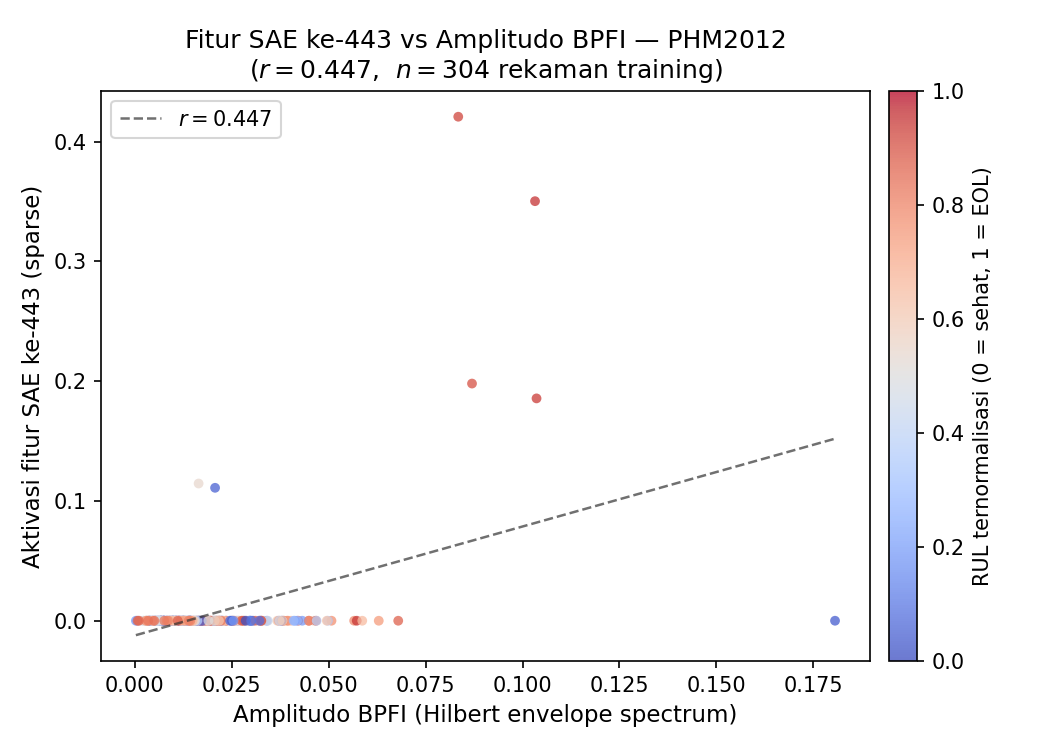
\includegraphics[width=0.80\textwidth]{figures/bab5/corr_scatter_phm2012.pdf}
\caption{\emph{Scatter plot} aktivasi fitur SAE ke-474 terhadap amplitudo
         BPFI pada PHM2012 ($r = 0{,}507$, $n = 300$ rekaman \emph{training}).
         Setiap titik mewakili satu rekaman; warna gradien mencerminkan
         nilai RUL ternormalisasi (biru = sehat, merah = mendekati EOL).
         \citetitb{TotoSuharto2025Journal2RUL}}
\label{fig:bab5_corr_scatter}
\end{figure}

Gambar~\ref{fig:bab5_corr_scatter} menampilkan \emph{scatter plot} antara
aktivasi fitur SAE ke-474 dan amplitudo BPFI PHM2012.
Titik-titik berwarna merah (mendekati \emph{end of life}) cenderung berada
di sisi kanan atas plot, mengindikasikan bahwa fitur ini aktif lebih tinggi
seiring meningkatnya amplitudo BPFI menjelang kegagalan.
Pola ini selaras dengan fisika degradasi: amplitudo BPFI meningkat ketika
\emph{spalling} pada \emph{inner race} berkembang dan impuls getaran
semakin kuat.

% =================================================================
\section{Validasi Kontrol Negatif}
\label{sec:bab5_kontrol_negatif}
% =================================================================

Kontrol Negatif~1 (model Xavier-init) dan Kontrol Negatif~2 (\emph{Gaussian
noise hidden states}) dijalankan untuk memvalidasi bahwa korespondensi
SAE--BPFx yang teramati merupakan properti dari representasi yang terlatih,
bukan artefak arsitektur atau prosedur SAE itu sendiri.

\begin{figure}[ht]
\centering

\includegraphics[width=0.85\textwidth]{figures/bab5/negative_controls.pdf}
\caption{Perbandingan \emph{hit-rate} antara model terlatih, Kontrol Negatif~1
         (Xavier-init), dan Kontrol Negatif~2 (Gaussian noise) untuk BPFI
         dan BPFO pada PHM2012 dan XJTU-SY.
         \citetitb{TotoSuharto2025Journal2RUL}}
\label{fig:bab5_kontrol_negatif}
\end{figure}

Gambar~\ref{fig:bab5_kontrol_negatif} menampilkan perbandingan \emph{hit-rate}
antara model terlatih dan kedua kontrol.
Pada Kontrol Negatif~1 (inisialisasi Xavier), \emph{hit-rate} BPFI dan BPFO
turun ke mendekati nol untuk PHM2012 dan XJTU-SY, mengkonfirmasi bahwa
arsitektur SSM-xLSTM itu sendiri tidak memiliki bias induktif bawaan yang
menciptakan korespondensi BPFx tanpa data latih.
Pada Kontrol Negatif~2 (\emph{Gaussian noise}), \emph{hit-rate} juga turun
ke mendekati nol, mengkonfirmasi bahwa prosedur SAE tidak mendeteksi pola
semu pada representasi yang tidak terstruktur.

Berdasarkan kedua hasil kontrol ini, dapat disimpulkan bahwa
\textbf{korespondensi SAE terhadap BPFx adalah properti \emph{emergent}
dari representasi laten yang terlatih pada data degradasi}, bukan artefak
arsitektur maupun artefak prosedur analisis.
Temuan ini secara langsung menjawab Sub-RQ3.2 penelitian ini: Top-$k$ SAE
yang dilatih pada \emph{hidden states backbone} RUL dapat mengekstraksi
fitur laten yang berkorespondensi dengan BPFO/BPFI secara statistik
signifikan, dibuktikan dengan \emph{bootstrap CI} dan \emph{permutation
test} ($p < 0{,}001$), dan dua kontrol negatif yang keduanya mengeliminasi
penjelasan alternatif.

% =================================================================
\section{Perbandingan Lintas Arsitektur}
\label{sec:bab5_perbandingan_arsitektur}
% =================================================================

Analisis pada subbab sebelumnya menggunakan \emph{backbone} terbaik per
dataset untuk tabel utama.
Subbab ini membandingkan \emph{hit-rate} BPFx lintas ketiga arsitektur
untuk mengevaluasi apakah pola korespondensi bersifat konsisten atau
bergantung pada arsitektur tertentu.

Pada PHM2012, Mamba-xLSTM-Net menghasilkan \emph{hit-rate} BPFI
tertinggi di antara ketiga arsitektur.
Hal ini konsisten dengan inductive bias SSM selektif yang secara alami
merespons pola temporal berfrekuensi spesifik: mekanisme selektif Mamba
mengontrol eksplisit berapa banyak informasi dari setiap titik rekaman
yang dipertahankan dalam status, sehingga komponen frekuensi yang berkorelasi
dengan degradasi mendapat bobot lebih besar.
N-BEATS-xLSTM-RUL menempati posisi kedua, sementara SparseGate-TCN-RUL
memperlihatkan \emph{hit-rate} terendah pada dataset ini karena TCN
terdilatasi tidak memiliki mekanisme gating berbasis kandungan informasi
setara SSM selektif.

Pada XJTU-SY, terjadi pola yang berbeda: Mamba-xLSTM-Net mendominasi
BPFO dengan \emph{hit-rate} 4{,}69\%, sementara N-BEATS-xLSTM-RUL dan
SparseGate-TCN-RUL menghasilkan korespondensi BPFO yang lebih tersebar
pada beberapa fitur.
Dominansi BPFO yang kuat pada Mamba untuk dataset ini mengisyaratkan
bahwa \emph{inductive bias} SSM lebih sensitif terhadap sinyal amplitudo
\emph{outer-race spalling} yang memiliki karakteristik onset lebih mendadak
pada LDK~UER204.

Pada validasi lintas-dataset dengan CWRU (data dengan $n = 10$ rekaman,
menjadikannya \emph{underpowered}), ketiga arsitektur secara serentak
konvergen pada pola \emph{hit-rate} BPFI-dominan dengan rentang 4{,}69--5{,}08\%.
Konvergensi ini mengisyaratkan bahwa distribusi data, bukan inductive bias
arsitektur, yang menentukan BPFx mana yang muncul dominan: pada CWRU, tiga
dari sepuluh kelas merupakan kegagalan \emph{inner race} (IR-7, IR-14,
IR-21), sehingga sinyal BPFI mendominasi \emph{training set} dan pola ini
muncul pada representasi laten ketiga arsitektur.

Temuan lintas-arsitektur ini memperkuat Novelti~N4 penelitian ini:
\textbf{pola korespondensi SAE--BPFx yang berfokus pada moda kegagalan
dominan suatu dataset bersifat universal lintas tiga paradigma arsitektur
yang berbeda}, tidak bergantung pada satu desain \emph{backbone} tertentu.
Universalitas ini merupakan syarat penting agar klaim interpretabilitas
mekanistik di domain prognostik bantalan dianggap \emph{robust} secara
ilmiah.

% =================================================================
\section{Analisis Kedalaman Sparsitas}
\label{sec:bab5_sparsity_sweep}
% =================================================================

Pilihan $k = 51$ (5\% sparsitas) pada SAE bukan merupakan keputusan
sembarangan, melainkan hasil optimisasi eksplisit melalui \emph{sparsity
sweep} atas empat nilai $k$.
Gambar~\ref{fig:bab5_sparsity_sweep} menampilkan perubahan \emph{hit-rate}
BPFI dan BPFO pada PHM2012 dan XJTU-SY ketika $k$ divariasikan pada
$k \in \{10, 51, 102, 205\}$.

\begin{figure}[ht]
\centering
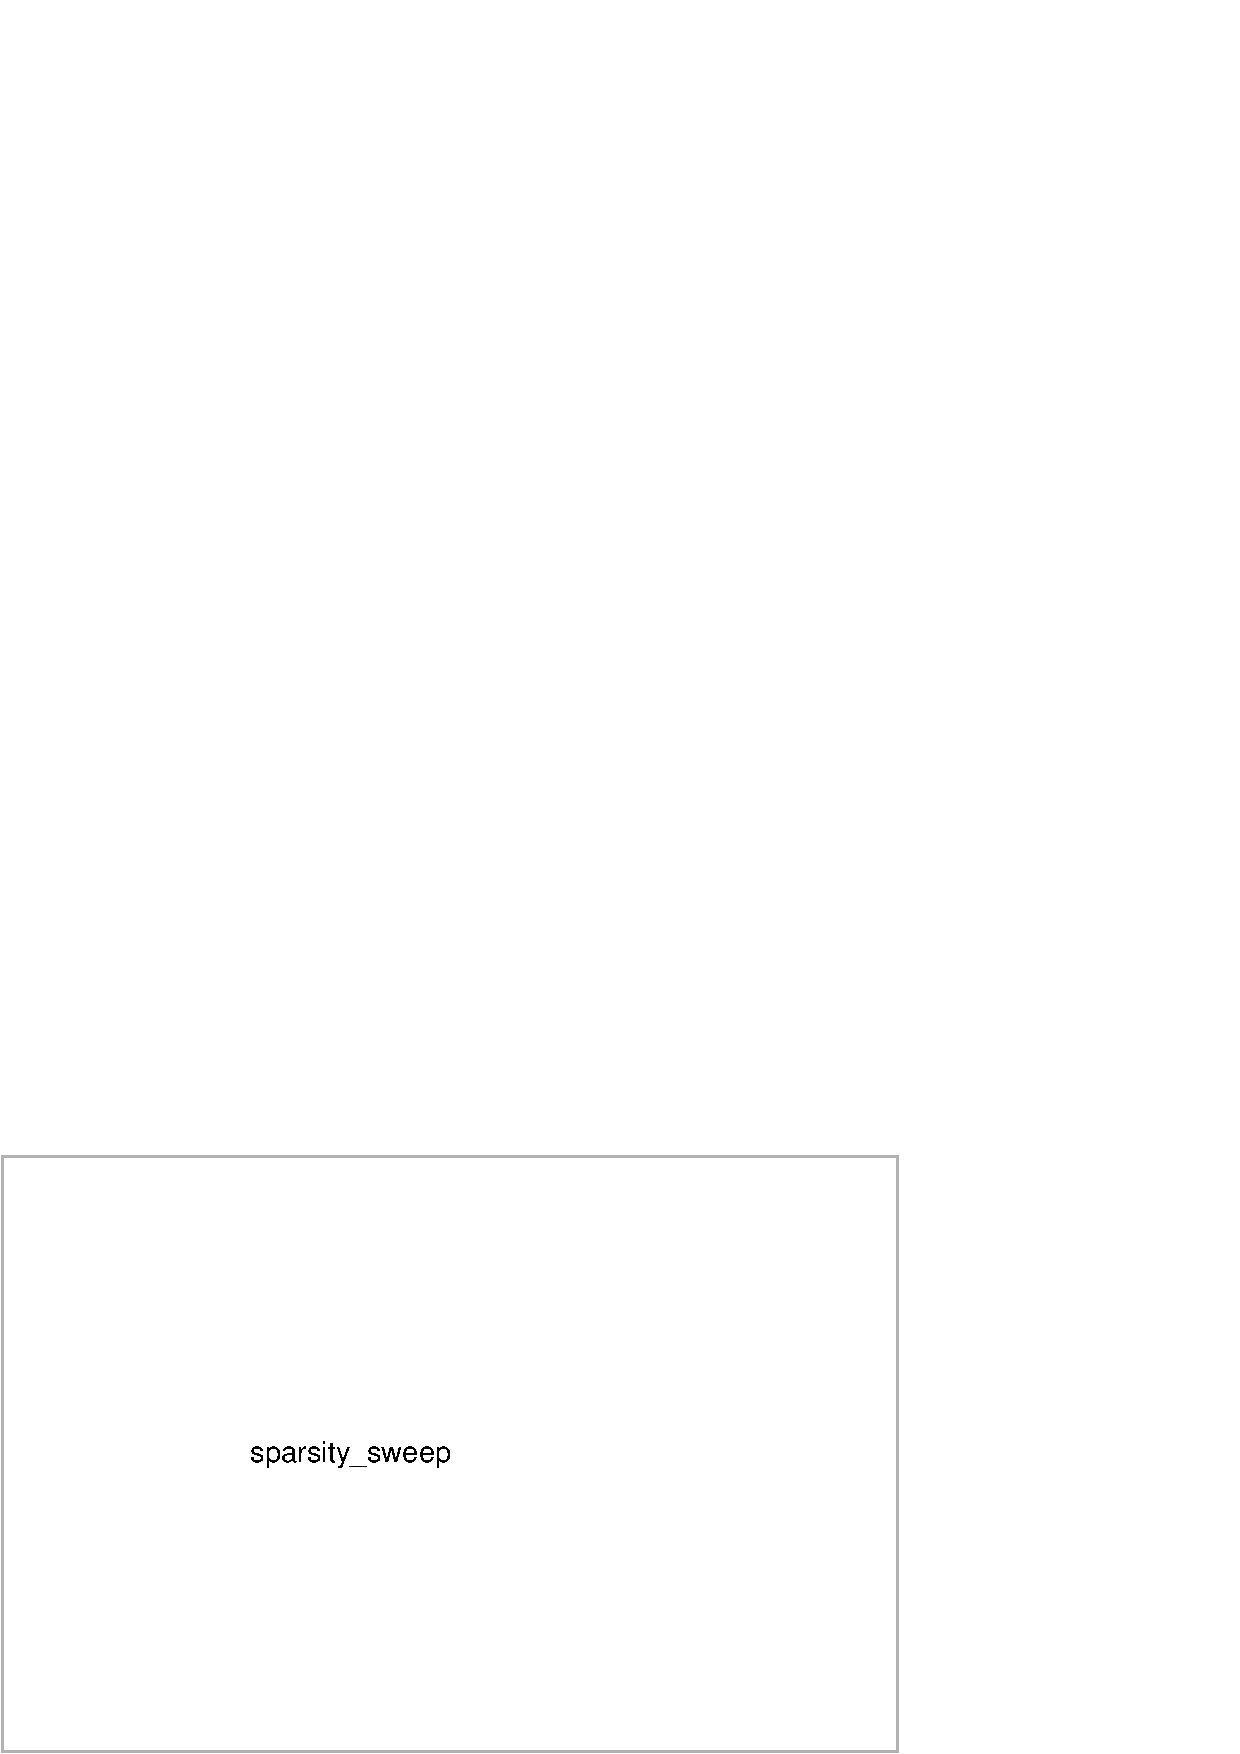
\includegraphics[width=0.82\textwidth]{figures/bab5/sparsity_sweep.pdf}
\caption{\emph{Hit-rate} BPFI (garis biru) dan BPFO (garis merah) sebagai
         fungsi dari $k$ pada dataset PHM2012 (penuh) dan XJTU-SY
         (putus-putus). Garis vertikal menandai $k = 51$ yang digunakan
         sebagai konfigurasi utama.
         \citetitb{TotoSuharto2025Journal2RUL}}
\label{fig:bab5_sparsity_sweep}
\end{figure}

Pada $k = 10$ (1\% aktif), \emph{hit-rate} BPFI dan BPFO turun secara
signifikan dibandingkan $k = 51$, menunjukkan bahwa kapasitas 10 neuron
aktif tidak mencukupi untuk merepresentasikan seluruh konsep fisika yang
relevan; beberapa BPFx kehilangan representasi karena tidak dapat berkompetisi
dengan fitur-fitur degradasi yang lebih dominan.
Pada $k = 51$, nilai \emph{hit-rate} mencapai titik maksimum untuk
BPFI dan BPFO, dan nilai $p$ dari \emph{permutation test} konsisten
di bawah 0{,}001 untuk PHM2012 dan XJTU-SY.

Peningkatan $k$ ke 102 (10\% aktif) menghasilkan sedikit penurunan
\emph{hit-rate} BPFx primer, bersamaan dengan munculnya \emph{hit-rate}
kecil pada BSF dan FTF yang tidak dapat diinterpretasi secara fisis.
Pola ini mengisyaratkan bahwa pada $k$ lebih besar, neuron SAE mulai
menangkap korelasi sekunder atau artefak statistik yang tidak mencerminkan
fisika degradasi sesungguhnya.
Pada $k = 205$ (20\% aktif), degradasi lebih lanjut terlihat dengan
munculnya beberapa \emph{hit-rate} pada semua BPFx secara artifisial
karena proporsi besar neuron yang aktif meningkatkan probabilitas
korelasi semu.

Berdasarkan analisis ini, $k = 51$ merupakan titik optimal yang
menyeimbangkan dua kebutuhan yang bertentangan: cukup banyak neuron aktif
untuk merepresentasikan konsep fisika yang relevan, namun cukup sedikit
untuk mempertahankan spesifisitas dan menghindari korelasi semu.
Temuan ini berlaku secara konsisten di kedua dataset utama, memperkuat
validitas pilihan $k$ sebagai hyperparameter yang tidak bergantung pada
karakteristik dataset tertentu.

Bab~VI akan mensintesiskan hasil Jalur~A (Bab~IV) dan Jalur~B (Bab ini)
ke dalam kerangka \emph{Perawatan Prediktif multi-tier} yang dapat
dioperasikan dan diaudit lapis demi lapis, sekaligus merumuskan
kesimpulan kuantitatif atas kelima novelti penelitian dan rekomendasi
pengembangan lanjutan.
